\documentclass[11pt]{article}

\usepackage[margin=1in]{geometry}
\usepackage[T1]{fontenc}
\usepackage{graphicx}
\usepackage{longtable}
\usepackage{booktabs}
\usepackage{array}
\usepackage{enumitem}
\usepackage{xcolor}
\usepackage{hyperref}
\usepackage{tikz}
\usepackage{float}
\usepackage{fancyhdr}
\usepackage{titlesec}
\usepackage{tcolorbox}
\usepackage{tabularx}
\usepackage{multirow}
\usepackage{caption}
\usepackage{listings}
\usepackage{makecell}
\usepackage{amssymb}
\usepackage{pifont}

\usetikzlibrary{shapes.geometric, arrows.meta, positioning, fit, backgrounds, calc, decorations.pathreplacing, shapes.multipart, matrix, shadows}

% ---------------------------------------------------------------------------
% Color Definitions
% ---------------------------------------------------------------------------
\definecolor{sectionblue}{RGB}{31,78,121}
\definecolor{devcolor}{RGB}{70,130,180}
\definecolor{testcolor}{RGB}{60,179,113}
\definecolor{plancolor}{RGB}{255,165,0}
\definecolor{flowcolor}{RGB}{100,100,100}
\definecolor{lightgray}{RGB}{245,245,245}
\definecolor{warningred}{RGB}{220,53,69}
\definecolor{successgreen}{RGB}{40,167,69}
\definecolor{infoblue}{RGB}{23,162,184}
\definecolor{integcolor}{RGB}{186,85,211}
\definecolor{qacolor}{RGB}{255,127,80}
\definecolor{deploycolor}{RGB}{144,238,144}
\definecolor{conformcolor}{RGB}{255,182,193}

\hypersetup{
  colorlinks=true,
  linkcolor=sectionblue,
  urlcolor=sectionblue,
  citecolor=sectionblue
}

% ---------------------------------------------------------------------------
% Header and Footer
% ---------------------------------------------------------------------------
\pagestyle{fancy}
\fancyhf{}
\fancyhead[L]{\leftmark}
\fancyhead[R]{Supporting Development Guide}
\fancyfoot[C]{\thepage}
\renewcommand{\headrulewidth}{0.4pt}
\renewcommand{\footrulewidth}{0.4pt}

% Avoid fancyhdr headheight warnings
\setlength{\headheight}{14pt}
\addtolength{\topmargin}{-2pt}


% ---------------------------------------------------------------------------
% Section Formatting
% ---------------------------------------------------------------------------
\titleformat{\section}
  {\normalfont\Large\bfseries\color{sectionblue}}{\thesection}{1em}{}
\titleformat{\subsection}
  {\normalfont\large\bfseries\color{sectionblue!80}}{\thesubsection}{1em}{}
\titleformat{\subsubsection}
  {\normalfont\normalsize\bfseries\color{sectionblue!60}}{\thesubsubsection}{1em}{}

% ---------------------------------------------------------------------------
% Custom Box Environments
% ---------------------------------------------------------------------------
\newtcolorbox{keypoint}{
    colback=blue!5,
    colframe=sectionblue,
    title=Key Point,
    fonttitle=\bfseries
}

\newtcolorbox{warning}{
    colback=red!5,
    colframe=warningred,
    title=Warning,
    fonttitle=\bfseries
}

\newtcolorbox{bestpractice}{
    colback=green!5,
    colframe=successgreen,
    title=Best Practice,
    fonttitle=\bfseries
}

\newtcolorbox{example}{
    colback=lightgray,
    colframe=flowcolor,
    title=Example,
    fonttitle=\bfseries
}

\newtcolorbox{definition}{
    colback=infoblue!10,
    colframe=infoblue,
    title=Definition,
    fonttitle=\bfseries
}

\newtcolorbox{questionbox}[1][]{
    colback=plancolor!10,
    colframe=plancolor,
    title=#1,
    fonttitle=\bfseries,
    breakable
}

\newtcolorbox{devbox}[1][]{
    colback=devcolor!10,
    colframe=devcolor,
    title=#1,
    fonttitle=\bfseries,
    breakable
}

\newtcolorbox{testbox}[1][]{
    colback=testcolor!10,
    colframe=testcolor,
    title=#1,
    fonttitle=\bfseries
}

\newtcolorbox{checklistbox}[1][]{
    colback=white,
    colframe=flowcolor,
    title=#1,
    fonttitle=\bfseries
}

\newtcolorbox{conformancebox}[1][]{
    colback=conformcolor!15,
    colframe=integcolor,
    title=#1,
    fonttitle=\bfseries
}

\tcbuselibrary{listings,breakable,skins}

% ---------------------------------------------------------------------------
% List Settings
% ---------------------------------------------------------------------------
\setlist[itemize]{leftmargin=*,topsep=3pt,itemsep=2pt,parsep=0pt}
\setlist[enumerate]{leftmargin=*,topsep=3pt,itemsep=2pt,parsep=0pt}

% ---------------------------------------------------------------------------
% Custom Column Types
% ---------------------------------------------------------------------------
\newcolumntype{L}[1]{>{\raggedright\arraybackslash}p{#1}}
\newcolumntype{C}[1]{>{\centering\arraybackslash}p{#1}}
\newcolumntype{R}[1]{>{\raggedleft\arraybackslash}p{#1}}

% ---------------------------------------------------------------------------
% Custom Commands
% ---------------------------------------------------------------------------
\newcommand{\AD}{architecture description}
\newcommand{\conform}{\textcolor{successgreen}{\ding{51}}}
\newcommand{\nonconform}{\textcolor{warningred}{\ding{55}}}
\newcommand{\partialmark}{\textcolor{plancolor}{\ding{72}}}

% ---------------------------------------------------------------------------
% Title
% ---------------------------------------------------------------------------
\title{%
    \vspace{-1cm}
    \textbf{\Huge Software Architecture Documentation}\\[12pt]
    \Large Supporting Development\\[8pt]
    \large A Comprehensive Guide to Using Architecture Documentation\\
    for Implementation, Testing, Integration, and Deployment
}
\author{%
    \textit{Architecture Documentation Series}\\[4pt]
    \small Based on SEI Views and Beyond and Industry Best Practices
}
\date{\today}

\begin{document}
\maketitle
\thispagestyle{empty}

\vspace{0.5cm}

\begin{abstract}
\noindent
Architecture documentation serves as the blueprint for system implementation. This comprehensive guide examines how architecture descriptions support the full development lifecycle---from project planning and resource estimation through implementation, testing, integration, and deployment. The document provides detailed question sets for each development stakeholder, checklists for assessing documentation readiness, and guidance for establishing conformance verification processes. Whether you are a software manager planning development resources, a developer implementing components, a tester designing test strategies, or an integrator planning system assembly, this guide ensures that architecture documentation provides the information you need to succeed.
\end{abstract}

\vfill

\begin{center}
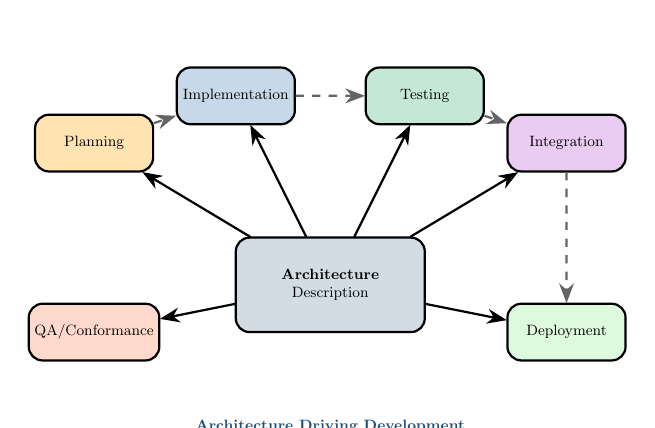
\begin{tikzpicture}[
    scale=0.6,
    transform shape,
    phase/.style={draw, thick, rounded corners=5pt, minimum width=2.5cm, minimum height=1.2cm, font=\small, align=center},
    arrow/.style={-{Stealth[length=2.5mm]}, thick}
]
    % Central AD
    \node[phase, fill=sectionblue!20, minimum width=4cm, minimum height=2cm] (ad) at (0,0) {\textbf{Architecture}\\Description};
    
    % Development phases
    \node[phase, fill=plancolor!30] (plan) at (-5,3) {Planning};
    \node[phase, fill=devcolor!30] (impl) at (-2,4) {Implementation};
    \node[phase, fill=testcolor!30] (test) at (2,4) {Testing};
    \node[phase, fill=integcolor!30] (integ) at (5,3) {Integration};
    \node[phase, fill=deploycolor!30] (deploy) at (5,-1) {Deployment};
    \node[phase, fill=qacolor!30] (qa) at (-5,-1) {QA/Conformance};
    
    % Connections
    \draw[arrow] (ad) -- (plan);
    \draw[arrow] (ad) -- (impl);
    \draw[arrow] (ad) -- (test);
    \draw[arrow] (ad) -- (integ);
    \draw[arrow] (ad) -- (deploy);
    \draw[arrow] (ad) -- (qa);
    
    % Flow between phases
    \draw[arrow, dashed, flowcolor] (plan) -- (impl);
    \draw[arrow, dashed, flowcolor] (impl) -- (test);
    \draw[arrow, dashed, flowcolor] (test) -- (integ);
    \draw[arrow, dashed, flowcolor] (integ) -- (deploy);
    
    % Label
    \node[font=\bfseries\small, text=sectionblue] at (0,-3) {Architecture Driving Development};
\end{tikzpicture}
\end{center}

\newpage
\tableofcontents
\newpage

%==============================================================================
\section{Introduction}
%==============================================================================

\subsection{Purpose of This Guide}

This guide examines how architecture documentation supports the software development lifecycle. Effective architecture documentation serves as a blueprint that enables development teams to:

\begin{itemize}
    \item Understand what to build and how components fit together
    \item Plan and estimate development resources accurately
    \item Implement components that conform to architectural intent
    \item Test systems against architectural requirements
    \item Integrate components into a working whole
    \item Deploy systems to production environments
    \item Verify conformance between implementation and architecture
\end{itemize}

\subsection{The Architecture-Development Relationship}

\begin{definition}
\textbf{Development Support:} The degree to which architecture documentation provides sufficient information for development stakeholders to perform their roles effectively and know when their work is complete.
\end{definition}

Architecture documentation bridges the gap between requirements and implementation. It provides the ``what'' and ``why'' that guide the ``how'' of implementation.

\begin{figure}[H]
\centering
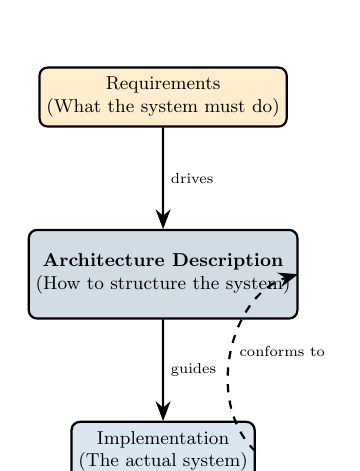
\begin{tikzpicture}[
    scale=0.75,
    transform shape,
    box/.style={draw, thick, rounded corners=3pt, minimum width=3cm, minimum height=1cm, font=\small, align=center},
    arrow/.style={-{Stealth[length=2.5mm]}, thick}
]
    \node[box, fill=plancolor!20] (req) at (0,3) {Requirements\\(What the system must do)};
    \node[box, fill=sectionblue!20, minimum width=4cm, minimum height=1.5cm] (arch) at (0,0) {\textbf{Architecture Description}\\(How to structure the system)};
    \node[box, fill=devcolor!20] (impl) at (0,-3) {Implementation\\(The actual system)};
    
    \draw[arrow] (req) -- node[right, font=\scriptsize] {drives} (arch);
    \draw[arrow] (arch) -- node[right, font=\scriptsize] {guides} (impl);
    \draw[arrow, dashed] (impl.east) to[bend left=60] node[right, font=\scriptsize] {conforms to} (arch.east);
\end{tikzpicture}
\caption{Architecture as Bridge Between Requirements and Implementation}
\end{figure}

\subsection{Stakeholder Overview}

Development support involves multiple stakeholder groups, each with distinct information needs:

\begin{longtable}{@{}L{3cm} L{4.5cm} L{5cm}@{}}
\caption{Development Stakeholders and Their Concerns} \\
\toprule
\textbf{Stakeholder} & \textbf{Primary Role} & \textbf{Key Information Needs} \\
\midrule
\endfirsthead
\toprule
\textbf{Stakeholder} & \textbf{Primary Role} & \textbf{Key Information Needs} \\
\midrule
\endhead
\bottomrule
\endlastfoot
Software Manager & Resource planning and scheduling & Implementation units; dependencies; effort estimates \\
Designer & Detailed design decisions & Constraints; patterns; interfaces; rationale \\
Implementer & Code development & Component specs; APIs; coding standards \\
Unit Tester & Component verification & Test criteria; dependencies; test data needs \\
Integrator & Component assembly & Integration order; interface contracts; runtime dependencies \\
System Tester & End-to-end verification & Test scenarios; quality requirements; acceptance criteria \\
QA/Conformance & Quality assurance & Conformance points; verification methods; traceability \\
Fielder/Deployer & Production deployment & Deployment topology; configuration; operational requirements \\
\end{longtable}

%==============================================================================
\section{Implementation Unit Identification}
%==============================================================================

\subsection{What is an Implementation Unit?}

\begin{definition}
An \textbf{implementation unit} is a portion of the system that can be assigned to a developer or team for implementation, has identifiable interfaces, can be separately compiled or built, and can be independently tested to some degree.
\end{definition}

The architecture documentation must clearly identify all implementation units and their relationships.

\subsection{Unit Identification from Architecture Views}

Different architectural views contribute to implementation unit identification:

\begin{longtable}{@{}L{3cm} L{4.5cm} L{5cm}@{}}
\caption{Views and Implementation Unit Information} \\
\toprule
\textbf{View Type} & \textbf{Unit Information} & \textbf{Development Use} \\
\midrule
\endfirsthead
\bottomrule
\endlastfoot
Module Decomposition & Code modules; packages; classes & Work breakdown; team assignment \\
Uses View & Module dependencies & Build order; impact analysis \\
Layered View & Layer membership; allowed dependencies & Dependency rules; portability \\
Component-Connector & Runtime components; connectors & Runtime behavior; communication \\
Deployment View & Nodes; allocation of components & Deployment planning; resource needs \\
Data Model View & Data entities; relationships & Database design; data access \\
\end{longtable}

\subsection{Implementation Unit Registry}

\begin{devbox}[Implementation Unit Registry Template]

\textbf{Unit ID:} [Unique identifier, e.g., IU-ORDER-001]

\textbf{Unit Name:} [Descriptive name]

\textbf{Description:} [Brief description of responsibility]

\textbf{Architecture Element:} [Reference to architectural element(s)]

\textbf{Type:} [Service / Library / Component / Module / Database / Configuration]

\textbf{Owner:} [Team or individual responsible]

\textbf{Dependencies:}
\begin{itemize}[nosep]
    \item Build-time: [Units required for compilation]
    \item Runtime: [Units required for execution]
    \item Test: [Units/resources required for testing]
\end{itemize}

\textbf{Interfaces:}
\begin{itemize}[nosep]
    \item Provided: [APIs/services this unit exposes]
    \item Required: [APIs/services this unit consumes]
\end{itemize}

\textbf{Quality Requirements:}
\begin{itemize}[nosep]
    \item Performance: [Response time, throughput targets]
    \item Reliability: [Availability, error handling requirements]
    \item Security: [Authentication, authorization requirements]
\end{itemize}

\textbf{Constraints:} [Technology, standards, patterns that must be followed]

\textbf{Estimated Effort:} [Story points / person-days / lines of code]

\textbf{Status:} [Not Started / In Progress / Code Complete / Tested / Integrated]
\end{devbox}

\subsection{Example Implementation Unit Catalog}

\begin{longtable}{@{}L{2cm} L{2.5cm} L{2.5cm} L{2cm} L{2cm} L{1.5cm}@{}}
\caption{Example Implementation Unit Catalog} \\
\toprule
\textbf{Unit ID} & \textbf{Name} & \textbf{Type} & \textbf{Owner} & \textbf{Build Deps} & \textbf{Effort} \\
\midrule
\endfirsthead
\bottomrule
\endlastfoot
IU-001 & Order Service & Service & Order Team & IU-010, IU-011 & 40 pts \\
IU-002 & Payment Service & Service & Payment Team & IU-010, IU-012 & 35 pts \\
IU-003 & Inventory Service & Service & Inventory Team & IU-010 & 30 pts \\
IU-004 & User Service & Service & Identity Team & IU-010, IU-012 & 25 pts \\
IU-005 & API Gateway & Component & Platform Team & IU-010 & 20 pts \\
IU-010 & Common Library & Library & Platform Team & -- & 15 pts \\
IU-011 & Messaging Library & Library & Platform Team & IU-010 & 10 pts \\
IU-012 & Security Library & Library & Security Team & IU-010 & 15 pts \\
IU-020 & Order Database & Database & DBA Team & -- & 10 pts \\
IU-021 & User Database & Database & DBA Team & -- & 8 pts \\
\end{longtable}

%==============================================================================
\section{Development Planning Support}
%==============================================================================

\subsection{Resource Estimation}

Architecture documentation should enable accurate resource estimation by providing:

\begin{itemize}
    \item Clear scope definition for each implementation unit
    \item Complexity indicators (interfaces, dependencies, quality requirements)
    \item Technology constraints affecting effort
    \item Reuse opportunities (existing components, libraries, patterns)
    \item Risk factors (new technology, complex integration, unclear requirements)
\end{itemize}

\begin{bestpractice}
\textbf{Estimation Guidance from Architecture:}

\begin{enumerate}
    \item \textbf{Count implementation units:} Establish baseline scope
    \item \textbf{Assess complexity:} Consider interfaces, dependencies, quality requirements
    \item \textbf{Identify reuse:} Reduce estimates for reused/adapted components
    \item \textbf{Add integration effort:} Account for component integration work
    \item \textbf{Include architecture-specific tasks:} Frameworks, infrastructure, cross-cutting concerns
    \item \textbf{Apply risk factors:} Adjust for uncertainty and technical risk
\end{enumerate}
\end{bestpractice}

\subsection{Dependency Analysis}

\begin{figure}[H]
\centering
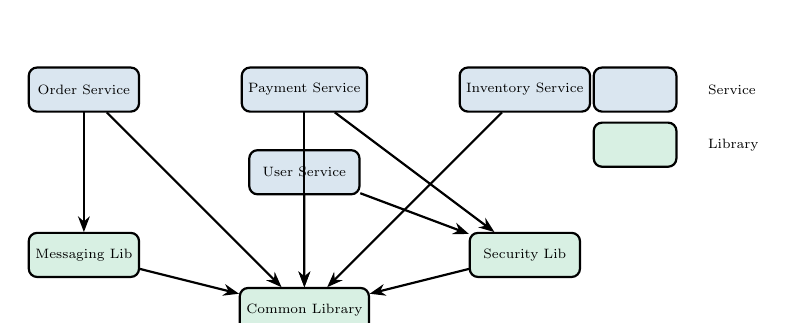
\begin{tikzpicture}[
    scale=0.7,
    transform shape,
    unit/.style={draw, thick, fill=devcolor!20, minimum width=2cm, minimum height=0.8cm, rounded corners=3pt, font=\scriptsize},
    lib/.style={draw, thick, fill=testcolor!20, minimum width=2cm, minimum height=0.8cm, rounded corners=3pt, font=\scriptsize},
    arrow/.style={-{Stealth[length=2mm]}, thick}
]
    % Services
    \node[unit] (order) at (0,3) {Order Service};
    \node[unit] (payment) at (4,3) {Payment Service};
    \node[unit] (inventory) at (8,3) {Inventory Service};
    \node[unit] (user) at (4,1.5) {User Service};
    
    % Libraries
    \node[lib] (common) at (4,-1) {Common Library};
    \node[lib] (messaging) at (0,0) {Messaging Lib};
    \node[lib] (security) at (8,0) {Security Lib};
    
    % Dependencies
    \draw[arrow] (order) -- (messaging);
    \draw[arrow] (order) -- (common);
    \draw[arrow] (payment) -- (common);
    \draw[arrow] (payment) -- (security);
    \draw[arrow] (inventory) -- (common);
    \draw[arrow] (user) -- (common);
    \draw[arrow] (user) -- (security);
    \draw[arrow] (messaging) -- (common);
    \draw[arrow] (security) -- (common);
    
    % Legend
    \node[unit, minimum width=1.5cm] at (10,3) {};
    \node[font=\scriptsize, right] at (11.2,3) {Service};
    \node[lib, minimum width=1.5cm] at (10,2) {};
    \node[font=\scriptsize, right] at (11.2,2) {Library};
\end{tikzpicture}
\caption{Build Dependency Graph}
\end{figure}

\subsection{Development Schedule Planning}

Architecture dependencies determine feasible development sequences:

\begin{longtable}{@{}L{2cm} L{3cm} L{3.5cm} L{4cm}@{}}
\caption{Development Phasing Based on Dependencies} \\
\toprule
\textbf{Phase} & \textbf{Units} & \textbf{Prerequisites} & \textbf{Parallel Opportunities} \\
\midrule
\endfirsthead
\bottomrule
\endlastfoot
Phase 1 & Common Library & None & Single unit \\
Phase 2 & Messaging Lib, Security Lib & Common Library & Both can be parallel \\
Phase 3 & Order, Payment, Inventory, User Services & Phase 2 complete & All services can be parallel \\
Phase 4 & API Gateway & Services available & Depends on service APIs \\
Phase 5 & Integration Testing & All units complete & -- \\
\end{longtable}

\subsection{Parallel Development Identification}

\begin{keypoint}
\textbf{Enabling Parallel Development:}

Architecture documentation enables parallel development when it clearly defines:

\begin{itemize}
    \item \textbf{Interface contracts:} Teams can work against defined interfaces before implementations exist
    \item \textbf{Dependency direction:} Lower-level components developed first or mocked
    \item \textbf{Integration points:} Clear handoff points between teams
    \item \textbf{Shared resources:} Coordination requirements for shared components
\end{itemize}
\end{keypoint}

%==============================================================================
\section{Design Guidance and Constraints}
%==============================================================================

\subsection{Architectural Constraints}

The architecture documentation should clearly communicate constraints that implementations must follow:

\begin{longtable}{@{}L{3cm} L{4.5cm} L{5cm}@{}}
\caption{Types of Architectural Constraints} \\
\toprule
\textbf{Constraint Type} & \textbf{Description} & \textbf{Examples} \\
\midrule
\endfirsthead
\toprule
\textbf{Constraint Type} & \textbf{Description} & \textbf{Examples} \\
\midrule
\endhead
\bottomrule
\endlastfoot
Technology & Required or prohibited technologies & ``Must use Java 17+''; ``No vendor-specific SQL'' \\
Dependency & Allowed/prohibited module dependencies & ``UI layer cannot access database directly'' \\
Communication & Required communication patterns & ``Services communicate via REST or events only'' \\
Data & Data management rules & ``Each service owns its data''; ``No shared databases'' \\
Security & Security requirements & ``All external APIs require authentication'' \\
Performance & Performance boundaries & ``Response time $<$500ms at p95'' \\
Pattern & Required design patterns & ``Use repository pattern for data access'' \\
Standard & Standards compliance & ``RESTful APIs follow OpenAPI 3.0'' \\
\end{longtable}

\subsection{Design Rules and Principles}

\begin{devbox}[Architectural Design Rules]

\textbf{Dependency Rules:}
\begin{enumerate}[nosep]
    \item Higher layers may depend on lower layers, not vice versa
    \item Domain layer has no external dependencies
    \item Infrastructure adapters depend on domain interfaces
    \item No circular dependencies between modules
\end{enumerate}

\textbf{Communication Rules:}
\begin{enumerate}[nosep]
    \item Synchronous calls only for queries; commands use async messaging
    \item All inter-service communication through defined APIs
    \item No direct database access across service boundaries
    \item Events published for all state changes
\end{enumerate}

\textbf{Data Rules:}
\begin{enumerate}[nosep]
    \item Each service owns its database schema
    \item No foreign keys across service boundaries
    \item Data replication via events, not shared tables
    \item Sensitive data encrypted at rest and in transit
\end{enumerate}

\textbf{Error Handling Rules:}
\begin{enumerate}[nosep]
    \item All exceptions logged with correlation ID
    \item Circuit breakers on all external calls
    \item Retry with exponential backoff for transient failures
    \item Graceful degradation when dependencies unavailable
\end{enumerate}
\end{devbox}

\subsection{Pattern and Style Guidance}

\begin{longtable}{@{}L{3cm} L{4cm} L{5.5cm}@{}}
\caption{Architectural Patterns and Their Application} \\
\toprule
\textbf{Pattern} & \textbf{When to Apply} & \textbf{Implementation Guidance} \\
\midrule
\endfirsthead
\bottomrule
\endlastfoot
Repository & Data access layer & Abstract data store; return domain objects \\
Factory & Complex object creation & Encapsulate construction logic \\
Strategy & Varying algorithms & Interface with multiple implementations \\
Observer/Event & State change notification & Event bus for loose coupling \\
Circuit Breaker & External service calls & Fail fast after threshold; auto-recover \\
Retry & Transient failures & Exponential backoff; max attempts \\
Saga & Distributed transactions & Compensating actions for rollback \\
CQRS & Read/write separation & Separate models for queries and commands \\
\end{longtable}

\subsection{Variability and Change Guidance}

Architecture documentation should identify what is likely to change and how to accommodate it:

\begin{longtable}{@{}L{3cm} L{4cm} L{5.5cm}@{}}
\caption{Change Accommodation Guidance} \\
\toprule
\textbf{Change Type} & \textbf{Architecture Provision} & \textbf{Implementation Approach} \\
\midrule
\endfirsthead
\bottomrule
\endlastfoot
New payment provider & Payment gateway abstraction & Implement new adapter; configure \\
Database migration & Repository pattern & Change repository implementation \\
UI framework change & Layered architecture & Replace UI layer only \\
New business rules & Rule engine / Strategy & Add new rule implementation \\
Scaling requirements & Stateless services & Horizontal scaling; no code change \\
New integration & API gateway / Adapters & Add new adapter; register route \\
\end{longtable}

%==============================================================================
\section{Testing Support}
%==============================================================================

\subsection{Architecture-Based Testing}

Architecture documentation supports testing by defining what to test, how to test it, and when testing is complete.

\begin{figure}[H]
\centering
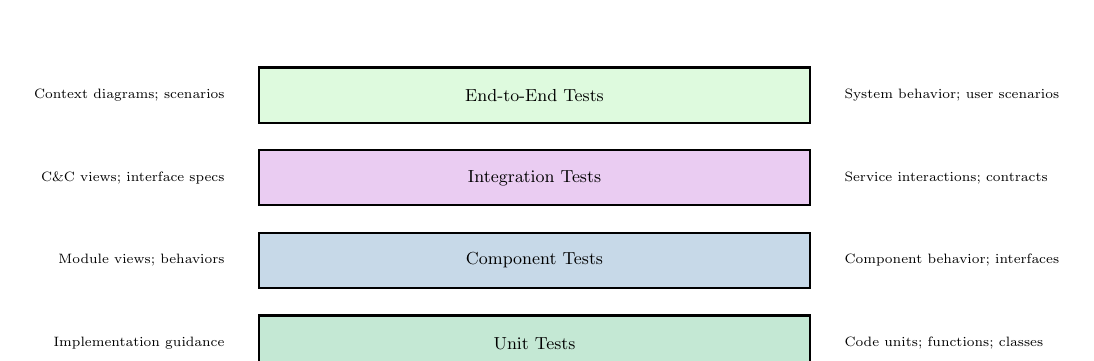
\begin{tikzpicture}[
    scale=0.7,
    transform shape,
    level/.style={draw, thick, fill=#1, minimum width=10cm, minimum height=1cm, font=\small},
    arrow/.style={-{Stealth[length=2mm]}, thick}
]
    \node[level=deploycolor!30] (e2e) at (0,4) {End-to-End Tests};
    \node[level=integcolor!30] (integ) at (0,2.5) {Integration Tests};
    \node[level=devcolor!30] (comp) at (0,1) {Component Tests};
    \node[level=testcolor!30] (unit) at (0,-0.5) {Unit Tests};
    
    % Annotations
    \node[font=\scriptsize, right] at (5.5,4) {System behavior; user scenarios};
    \node[font=\scriptsize, right] at (5.5,2.5) {Service interactions; contracts};
    \node[font=\scriptsize, right] at (5.5,1) {Component behavior; interfaces};
    \node[font=\scriptsize, right] at (5.5,-0.5) {Code units; functions; classes};
    
    % Architecture relevance
    \node[font=\scriptsize, left] at (-5.5,4) {Context diagrams; scenarios};
    \node[font=\scriptsize, left] at (-5.5,2.5) {C\&C views; interface specs};
    \node[font=\scriptsize, left] at (-5.5,1) {Module views; behaviors};
    \node[font=\scriptsize, left] at (-5.5,-0.5) {Implementation guidance};
\end{tikzpicture}
\caption{Test Pyramid and Architecture Documentation}
\end{figure}

\subsection{Test Information from Architecture}

\begin{testbox}[Architecture-Derived Test Information]

\textbf{From Module Views:}
\begin{itemize}[nosep]
    \item Unit boundaries for isolation testing
    \item Dependencies requiring mocks/stubs
    \item Internal interfaces for component testing
\end{itemize}

\textbf{From C\&C Views:}
\begin{itemize}[nosep]
    \item Service contracts for contract testing
    \item Communication paths for integration testing
    \item Runtime configurations for scenario testing
\end{itemize}

\textbf{From Behavior Descriptions:}
\begin{itemize}[nosep]
    \item Scenarios for end-to-end testing
    \item State transitions for state-based testing
    \item Error conditions for negative testing
\end{itemize}

\textbf{From Quality Requirements:}
\begin{itemize}[nosep]
    \item Performance targets for load testing
    \item Reliability requirements for chaos testing
    \item Security requirements for penetration testing
\end{itemize}

\textbf{From Deployment Views:}
\begin{itemize}[nosep]
    \item Environment configurations for deployment testing
    \item Resource requirements for capacity testing
    \item Network topology for failover testing
\end{itemize}
\end{testbox}

\subsection{Test Success Criteria}

\begin{longtable}{@{}L{2.5cm} L{4cm} L{6cm}@{}}
\caption{Architecture-Based Test Success Criteria} \\
\toprule
\textbf{Test Level} & \textbf{Success Criteria Source} & \textbf{Example Criteria} \\
\midrule
\endfirsthead
\bottomrule
\endlastfoot
Unit Test & Interface specifications & All public methods tested; edge cases covered \\
Component Test & Component behavior specs & All interfaces exercised; error paths tested \\
Integration Test & Interface contracts & Contracts verified; communication paths tested \\
System Test & Quality attribute scenarios & Performance targets met; security verified \\
Acceptance Test & Stakeholder scenarios & Use cases pass; business rules verified \\
\end{longtable}

\subsection{Test Environment Requirements}

Architecture documentation should specify test environment needs:

\begin{itemize}
    \item \textbf{Unit testing:} Minimal; mocks for dependencies
    \item \textbf{Component testing:} Component under test; stubbed dependencies
    \item \textbf{Integration testing:} Multiple components; test databases; message brokers
    \item \textbf{System testing:} Full environment; production-like data; external system simulators
    \item \textbf{Performance testing:} Scaled environment; load generators; monitoring
\end{itemize}

%==============================================================================
\section{Integration and Deployment Support}
%==============================================================================

\subsection{Integration Planning}

Architecture documentation supports integration by defining:

\begin{longtable}{@{}L{3cm} L{4.5cm} L{5cm}@{}}
\caption{Integration Information from Architecture} \\
\toprule
\textbf{Information} & \textbf{Source} & \textbf{Integration Use} \\
\midrule
\endfirsthead
\bottomrule
\endlastfoot
Integration units & Module decomposition & What must be integrated \\
Integration order & Dependency analysis & Sequence of integration \\
Interface contracts & Interface specifications & Verification criteria \\
Runtime dependencies & C\&C view & Resources needed for integration \\
Integration test cases & Behavior descriptions & How to verify integration \\
Configuration & Deployment view & Environment setup \\
\end{longtable}

\subsection{Integration Strategies}

\begin{devbox}[Architecture-Driven Integration Strategies]

\textbf{Bottom-Up Integration:}
\begin{itemize}[nosep]
    \item Start with lowest-level components (libraries, utilities)
    \item Progress upward through dependency layers
    \item Each level tested before moving up
    \item Requires drivers to test components
\end{itemize}

\textbf{Top-Down Integration:}
\begin{itemize}[nosep]
    \item Start with highest-level components
    \item Progressively integrate lower levels
    \item Uses stubs for unimplemented components
    \item Early validation of system structure
\end{itemize}

\textbf{Feature-Based Integration:}
\begin{itemize}[nosep]
    \item Integrate components needed for specific features
    \item Vertical slices through architecture
    \item Early delivery of working functionality
    \item May require both stubs and drivers
\end{itemize}

\textbf{Continuous Integration:}
\begin{itemize}[nosep]
    \item Integrate frequently (multiple times per day)
    \item Automated build and test
    \item Early detection of integration issues
    \item Requires robust test automation
\end{itemize}
\end{devbox}

\subsection{Deployment Information}

\begin{longtable}{@{}L{3cm} L{4.5cm} L{5cm}@{}}
\caption{Deployment Information from Architecture} \\
\toprule
\textbf{Information} & \textbf{Architecture Source} & \textbf{Deployment Use} \\
\midrule
\endfirsthead
\bottomrule
\endlastfoot
Deployment topology & Deployment view & Infrastructure provisioning \\
Component allocation & Deployment mapping & Where to deploy each component \\
Resource requirements & Quality attribute analysis & Sizing and capacity \\
Configuration & Variability guide & Environment-specific settings \\
Dependencies & Runtime dependencies & Deployment order; health checks \\
Network requirements & C\&C communication & Firewall rules; load balancers \\
\end{longtable}

\subsection{Deployment Checklist}

\begin{checklistbox}[Architecture-Based Deployment Checklist]

\textbf{Pre-Deployment:}
\begin{itemize}[leftmargin=1.5cm]
    \item[$\square$] All implementation units identified in architecture are built
    \item[$\square$] All integration tests pass
    \item[$\square$] Deployment topology matches architecture deployment view
    \item[$\square$] Configuration matches architecture specifications
    \item[$\square$] Resource allocation meets architecture requirements
\end{itemize}

\textbf{Deployment Verification:}
\begin{itemize}[leftmargin=1.5cm]
    \item[$\square$] All components deployed to correct nodes
    \item[$\square$] All communication paths operational
    \item[$\square$] All external integrations connected
    \item[$\square$] Health checks passing
    \item[$\square$] Monitoring and alerting configured
\end{itemize}

\textbf{Post-Deployment:}
\begin{itemize}[leftmargin=1.5cm]
    \item[$\square$] Smoke tests pass
    \item[$\square$] Performance within architecture targets
    \item[$\square$] Security controls verified
    \item[$\square$] Deployment documented
\end{itemize}
\end{checklistbox}

%==============================================================================
\section{Conformance Verification}
%==============================================================================

\subsection{What is Architectural Conformance?}

\begin{definition}
\textbf{Architectural Conformance:} The degree to which the implemented system adheres to the prescribed architecture. Conformance verification ensures that implementation decisions align with architectural intent.
\end{definition}

\subsection{Conformance Points}

Architecture documentation should identify specific conformance points---aspects of the implementation that must match the architecture:

\begin{longtable}{@{}L{3cm} L{4cm} L{5.5cm}@{}}
\caption{Conformance Point Categories} \\
\toprule
\textbf{Category} & \textbf{Conformance Points} & \textbf{Verification Method} \\
\midrule
\endfirsthead
\toprule
\textbf{Category} & \textbf{Conformance Points} & \textbf{Verification Method} \\
\midrule
\endhead
\bottomrule
\endlastfoot
Structure & Module decomposition matches architecture & Static analysis; code review \\
Dependencies & Only allowed dependencies exist & Dependency analysis tools \\
Interfaces & APIs match specifications & Contract testing; API comparison \\
Behavior & Runtime behavior matches scenarios & Integration testing; monitoring \\
Quality & Quality targets met & Performance testing; security scanning \\
Deployment & Deployment matches topology & Infrastructure inspection \\
Standards & Coding standards followed & Linting; static analysis \\
Patterns & Required patterns implemented & Code review; architecture fitness functions \\
\end{longtable}

\subsection{Conformance Verification Methods}

\begin{conformancebox}[Conformance Verification Approaches]

\textbf{Static Analysis:}
\begin{itemize}[nosep]
    \item Dependency checking (forbidden dependencies)
    \item Layer violation detection
    \item Coding standard enforcement
    \item Architecture rule checking
\end{itemize}

\textbf{Dynamic Analysis:}
\begin{itemize}[nosep]
    \item Runtime behavior verification
    \item Performance measurement
    \item Communication pattern verification
    \item Resource usage monitoring
\end{itemize}

\textbf{Manual Review:}
\begin{itemize}[nosep]
    \item Architecture review boards
    \item Code reviews with architecture focus
    \item Design document reviews
    \item Deployment verification
\end{itemize}

\textbf{Architecture Fitness Functions:}
\begin{itemize}[nosep]
    \item Automated architecture tests
    \item Continuous conformance checking
    \item Metrics and thresholds
    \item Build pipeline integration
\end{itemize}
\end{conformancebox}

\subsection{Conformance Verification Process}

\begin{figure}[H]
\centering
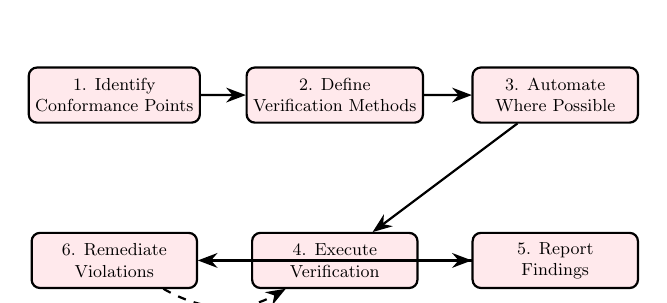
\begin{tikzpicture}[
    scale=0.7,
    transform shape,
    stepbox/.style={draw, thick, fill=conformcolor!30, minimum width=3cm, minimum height=1cm, rounded corners=3pt, font=\small, align=center},
    arrow/.style={-{Stealth[length=2.5mm]}, thick}
]
    \node[stepbox] (identify) at (0,4) {1. Identify\\Conformance Points};
    \node[stepbox] (method) at (4,4) {2. Define\\Verification Methods};
    \node[stepbox] (automate) at (8,4) {3. Automate\\Where Possible};
    \node[stepbox] (execute) at (4,1) {4. Execute\\Verification};
    \node[stepbox] (report) at (8,1) {5. Report\\Findings};
    \node[stepbox] (remediate) at (0,1) {6. Remediate\\Violations};
    
    \draw[arrow] (identify) -- (method);
    \draw[arrow] (method) -- (automate);
    \draw[arrow] (automate) -- (execute);
    \draw[arrow] (execute) -- (report);
    \draw[arrow] (report) -- (remediate);
    \draw[arrow, dashed] (remediate) to[bend right=30] (execute);
\end{tikzpicture}
\caption{Conformance Verification Process}
\end{figure}

%==============================================================================
\section{Quality Assurance Support}
%==============================================================================

\subsection{QA Information Needs}

QA stakeholders require specific information from architecture documentation:

\begin{longtable}{@{}L{3.5cm} L{4cm} L{5cm}@{}}
\caption{QA Information Requirements} \\
\toprule
\textbf{QA Activity} & \textbf{Required Information} & \textbf{Architecture Source} \\
\midrule
\endfirsthead
\bottomrule
\endlastfoot
Baseline management & Version; status; change history & Document control section \\
Decision tracking & Key decisions; rationale & Rationale documentation \\
Traceability & Requirements to architecture mapping & Traceability matrices \\
Conformance planning & Conformance points; methods & Conformance specification \\
Issue management & Open issues; deferred decisions & Open issues section \\
Test alignment & Test approach consistency & Behavior descriptions \\
\end{longtable}

\subsection{Architecture Baselining}

\begin{bestpractice}
\textbf{Architecture Baseline Requirements:}

\begin{enumerate}
    \item \textbf{Version identification:} Clear version number and date
    \item \textbf{Status indication:} Draft/Review/Approved/Deprecated
    \item \textbf{Change history:} Record of all changes with rationale
    \item \textbf{Approval record:} Who approved and when
    \item \textbf{Distribution list:} Who has received the baseline
    \item \textbf{Configuration control:} How changes are managed
\end{enumerate}
\end{bestpractice}

\subsection{Open Decisions and Deferred Items}

Architecture documentation should clearly identify:

\begin{itemize}
    \item \textbf{Open decisions:} Architectural questions not yet resolved
    \item \textbf{Deferred decisions:} Decisions intentionally left to implementation
    \item \textbf{Known issues:} Problems or limitations in the architecture
    \item \textbf{Technical debt:} Shortcuts that need future attention
    \item \textbf{Assumptions:} Assumptions that may need validation
\end{itemize}

\begin{longtable}{@{}L{1.5cm} L{3.5cm} L{3cm} L{2cm} L{2.5cm}@{}}
\caption{Open Items Tracking} \\
\toprule
\textbf{ID} & \textbf{Description} & \textbf{Type} & \textbf{Impact} & \textbf{Resolution} \\
\midrule
\endfirsthead
\bottomrule
\endlastfoot
OI-001 & Cache eviction strategy & Deferred & Medium & Implementer choice \\
OI-002 & Multi-region deployment & Open & High & Q3 decision \\
OI-003 & Legacy API deprecation & Known Issue & Medium & Migration plan needed \\
OI-004 & Database sharding approach & Open & High & Performance testing \\
\end{longtable}

%==============================================================================
\section{Review Question Sets}
%==============================================================================

\subsection{Questions for Software Managers}

\begin{questionbox}[Software Manager Questions]

\textbf{Implementation Unit Identification:}
\begin{enumerate}
    \item Can you identify the complete set of implementation units from the architecture documentation?
    \item Is each unit clearly defined with scope and boundaries?
    \item Are unit ownership and responsibilities clearly assigned?
\end{enumerate}

\textbf{Resource Planning:}
\begin{enumerate}[resume]
    \item Can you estimate development effort for each unit?
    \item Are complexity factors (interfaces, quality requirements) documented?
    \item Can you identify reuse opportunities that reduce effort?
    \item Are there risk factors that affect estimates?
\end{enumerate}

\textbf{Dependency Management:}
\begin{enumerate}[resume]
    \item Can you determine build dependencies between units?
    \item Can you identify runtime dependencies?
    \item Are dependency directions clear (what depends on what)?
\end{enumerate}

\textbf{Schedule Planning:}
\begin{enumerate}[resume]
    \item Can you lay out a development schedule based on dependencies?
    \item Can you identify units that can be developed in parallel?
    \item Can you plan for architecture prototype/proof of concept?
    \item Are milestone criteria defined?
\end{enumerate}

\textbf{Constraint Assessment:}
\begin{enumerate}[resume]
    \item Does the architecture overconstrain developers unnecessarily?
    \item Are constraints clearly justified with rationale?
    \item Is there appropriate flexibility for implementation decisions?
\end{enumerate}
\end{questionbox}

\subsection{Questions for Designers and Implementers}

\begin{questionbox}[Designer/Implementer Questions]

\textbf{Dependency Understanding:}
\begin{enumerate}
    \item Can you identify allowed dependencies for your unit?
    \item Can you identify prohibited dependencies?
    \item Are dependency rules clearly documented and justified?
\end{enumerate}

\textbf{Constraints and Patterns:}
\begin{enumerate}[resume]
    \item Can you identify applicable architectural constraints?
    \item Are required patterns and styles documented?
    \item Is guidance provided for pattern application?
    \item Are technology constraints clear?
\end{enumerate}

\textbf{Requirements Traceability:}
\begin{enumerate}[resume]
    \item Can you navigate from your unit to its requirements?
    \item Are quality requirements for your unit clear?
    \item Are derived requirements documented?
\end{enumerate}

\textbf{Cross-Cutting Concerns:}
\begin{enumerate}[resume]
    \item Is error handling approach defined?
    \item Is resource management approach defined?
    \item Is data persistence approach defined?
    \item Is security implementation approach defined?
    \item Is logging and monitoring approach defined?
\end{enumerate}

\textbf{Change and Evolution:}
\begin{enumerate}[resume]
    \item Can you identify what is likely to change?
    \item Is impact of changes on your design clear?
    \item Are variation points documented?
    \item Is decision stability indicated (firm vs. tentative)?
\end{enumerate}

\textbf{Conformance:}
\begin{enumerate}[resume]
    \item Do you understand how conformance will be verified?
    \item Are conformance points for your unit identified?
    \item Do you know when your implementation is complete?
\end{enumerate}
\end{questionbox}

\subsection{Questions for Integrators and Fielders}

\begin{questionbox}[Integrator/Fielder Questions]

\textbf{Integration Planning:}
\begin{enumerate}
    \item Can you identify all units requiring integration?
    \item Is integration order determinable from dependencies?
    \item Are interface contracts defined for integration verification?
\end{enumerate}

\textbf{Resource Requirements:}
\begin{enumerate}[resume]
    \item Can you determine resources needed for each unit?
    \item Are runtime dependencies clearly documented?
    \item Is infrastructure requirements documented?
\end{enumerate}

\textbf{Integration Testing:}
\begin{enumerate}[resume]
    \item Are integration test obligations defined?
    \item Is integration success criteria clear?
    \item Are integration test environments specified?
\end{enumerate}

\textbf{Deployment Planning:}
\begin{enumerate}[resume]
    \item Is deployment topology clearly defined?
    \item Are configuration requirements documented?
    \item Is deployment order specified?
    \item Are rollback procedures defined?
\end{enumerate}

\textbf{Conformance:}
\begin{enumerate}[resume]
    \item Do you understand deployment conformance criteria?
    \item Are operational conformance points identified?
\end{enumerate}
\end{questionbox}

\subsection{Questions for Testers}

\begin{questionbox}[Tester Questions]

\textbf{Test Isolation:}
\begin{enumerate}
    \item Can you identify units testable in isolation?
    \item Are dependencies for isolated testing documented?
    \item Is mock/stub guidance provided?
\end{enumerate}

\textbf{Test Requirements:}
\begin{enumerate}[resume]
    \item For each unit, what data is needed for testing?
    \item What special hardware or infrastructure is needed?
    \item What other units must be available?
\end{enumerate}

\textbf{Test Success Criteria:}
\begin{enumerate}[resume]
    \item Are test success criteria defined for each unit?
    \item Are quality attribute targets testable?
    \item Are acceptance criteria defined?
\end{enumerate}

\textbf{System Testing:}
\begin{enumerate}[resume]
    \item Can the system be tested as a whole?
    \item Are end-to-end scenarios documented?
    \item Are system test environments specified?
\end{enumerate}
\end{questionbox}

\subsection{Questions for QA Stakeholders}

\begin{questionbox}[QA Stakeholder Questions]

\textbf{Baseline and History:}
\begin{enumerate}
    \item Is the architecture documentation baselined?
    \item Is change history maintained?
    \item Are versions clearly identified?
\end{enumerate}

\textbf{Decisions and Rationale:}
\begin{enumerate}[resume]
    \item Are key decisions identified?
    \item Is rationale captured for decisions?
    \item Are open decisions documented?
    \item Are deferred decisions clearly marked?
\end{enumerate}

\textbf{Traceability:}
\begin{enumerate}[resume]
    \item Is there traceability to requirements?
    \item Is there traceability to test artifacts?
    \item Is there traceability to implementation artifacts?
\end{enumerate}

\textbf{Consistency:}
\begin{enumerate}[resume]
    \item Are known inconsistencies documented?
    \item Are view-to-view correspondences defined?
    \item Are model-to-artifact mappings documented?
\end{enumerate}

\textbf{Conformance Process:}
\begin{enumerate}[resume]
    \item Are conformance points identified?
    \item Is there a documented conformance verification method?
    \item Does the architecture content support conformance checking?
    \item Is there a formal conformance process?
\end{enumerate}

\textbf{Issue Management:}
\begin{enumerate}[resume]
    \item How are developer issues captured?
    \item How are issues resolved and reflected in the architecture?
    \item Is there a feedback loop from implementation to architecture?
\end{enumerate}
\end{questionbox}

\subsection{Questions for All Stakeholders}

\begin{questionbox}[Universal Questions]

\begin{enumerate}
    \item Can you identify open, partially resolved, or unresolved issues in the architecture documentation?
    
    \item Are there areas of the architecture that are unclear or ambiguous?
    
    \item Can you identify where automated tools will be used in development?
    
    \item Does the architecture documentation have content in formats processable by tools?
    
    \item Is the architecture documentation accessible and navigable?
    
    \item Can you find the information you need without excessive searching?
    
    \item Is terminology used consistently throughout the documentation?
    
    \item Are cross-references accurate and helpful?
\end{enumerate}
\end{questionbox}

%==============================================================================
\section{Development Readiness Assessment}
%==============================================================================

\subsection{Readiness Checklist}

\begin{checklistbox}[Architecture Documentation Development Readiness]

\textbf{Implementation Unit Identification:}
\begin{itemize}[leftmargin=1.5cm]
    \item[$\square$] All implementation units identified
    \item[$\square$] Unit boundaries and responsibilities defined
    \item[$\square$] Unit ownership assigned
    \item[$\square$] Effort estimates possible
\end{itemize}

\textbf{Dependency Documentation:}
\begin{itemize}[leftmargin=1.5cm]
    \item[$\square$] Build dependencies documented
    \item[$\square$] Runtime dependencies documented
    \item[$\square$] Dependency rules and constraints defined
    \item[$\square$] Development sequence determinable
\end{itemize}

\textbf{Design Guidance:}
\begin{itemize}[leftmargin=1.5cm]
    \item[$\square$] Architectural constraints documented
    \item[$\square$] Required patterns identified
    \item[$\square$] Technology constraints specified
    \item[$\square$] Cross-cutting concern approaches defined
\end{itemize}

\textbf{Interface Specifications:}
\begin{itemize}[leftmargin=1.5cm]
    \item[$\square$] External interfaces specified
    \item[$\square$] Internal interfaces defined
    \item[$\square$] Interface contracts documented
    \item[$\square$] Data formats specified
\end{itemize}

\textbf{Quality Requirements:}
\begin{itemize}[leftmargin=1.5cm]
    \item[$\square$] Performance requirements allocated
    \item[$\square$] Security requirements allocated
    \item[$\square$] Other quality requirements allocated
    \item[$\square$] Test criteria defined
\end{itemize}

\textbf{Conformance Definition:}
\begin{itemize}[leftmargin=1.5cm]
    \item[$\square$] Conformance points identified
    \item[$\square$] Verification methods defined
    \item[$\square$] Completion criteria established
\end{itemize}

\textbf{Documentation Quality:}
\begin{itemize}[leftmargin=1.5cm]
    \item[$\square$] Documentation baselined
    \item[$\square$] Terminology consistent
    \item[$\square$] Cross-references accurate
    \item[$\square$] Open issues documented
\end{itemize}
\end{checklistbox}

\subsection{Readiness Assessment Matrix}

\begin{longtable}{@{}L{3cm} C{2cm} C{2cm} C{2cm} L{3.5cm}@{}}
\caption{Development Readiness Assessment} \\
\toprule
\textbf{Criterion} & \textbf{Ready} & \textbf{Partial} & \textbf{Not Ready} & \textbf{Notes} \\
\midrule
\endfirsthead
\bottomrule
\endlastfoot
Unit identification & $\square$ & $\square$ & $\square$ & \\
Dependencies & $\square$ & $\square$ & $\square$ & \\
Constraints & $\square$ & $\square$ & $\square$ & \\
Interfaces & $\square$ & $\square$ & $\square$ & \\
Quality requirements & $\square$ & $\square$ & $\square$ & \\
Test criteria & $\square$ & $\square$ & $\square$ & \\
Conformance points & $\square$ & $\square$ & $\square$ & \\
Rationale & $\square$ & $\square$ & $\square$ & \\
Documentation baseline & $\square$ & $\square$ & $\square$ & \\
\midrule
\textbf{Overall Assessment} & $\square$ & $\square$ & $\square$ & \\
\end{longtable}

%==============================================================================
\section{Appendix A: Implementation Unit Template}
%==============================================================================

\begin{devbox}[Detailed Implementation Unit Specification]

\textbf{1. Identification}
\begin{itemize}[nosep]
    \item Unit ID: [IU-XXX-NNN]
    \item Unit Name: [Descriptive name]
    \item Version: [X.Y.Z]
    \item Status: [Planned / In Development / Complete]
\end{itemize}

\textbf{2. Architecture Mapping}
\begin{itemize}[nosep]
    \item Module View Element: [Reference]
    \item C\&C View Element: [Reference]
    \item Deployment View Element: [Reference]
\end{itemize}

\textbf{3. Responsibility}
\begin{itemize}[nosep]
    \item Primary Responsibility: [Main purpose]
    \item Secondary Responsibilities: [Additional duties]
    \item Out of Scope: [What this unit does NOT do]
\end{itemize}

\textbf{4. Dependencies}
\begin{itemize}[nosep]
    \item Build Dependencies: [Required for compilation]
    \item Runtime Dependencies: [Required for execution]
    \item Test Dependencies: [Required for testing]
    \item Optional Dependencies: [Enhanced functionality]
\end{itemize}

\textbf{5. Interfaces}
\begin{itemize}[nosep]
    \item Provided Interfaces: [APIs exposed]
    \item Required Interfaces: [APIs consumed]
    \item Events Published: [Events emitted]
    \item Events Subscribed: [Events handled]
\end{itemize}

\textbf{6. Quality Requirements}
\begin{itemize}[nosep]
    \item Performance: [Specific targets]
    \item Availability: [Uptime requirements]
    \item Security: [Security requirements]
    \item Other: [Additional quality requirements]
\end{itemize}

\textbf{7. Constraints}
\begin{itemize}[nosep]
    \item Technology: [Required technologies]
    \item Standards: [Standards to follow]
    \item Patterns: [Required patterns]
\end{itemize}

\textbf{8. Test Criteria}
\begin{itemize}[nosep]
    \item Unit Test Coverage: [Target percentage]
    \item Integration Test Scenarios: [Key scenarios]
    \item Performance Test Criteria: [Targets]
\end{itemize}

\textbf{9. Conformance Points}
\begin{itemize}[nosep]
    \item Structure: [Conformance checks]
    \item Behavior: [Conformance checks]
    \item Quality: [Conformance checks]
\end{itemize}
\end{devbox}

%==============================================================================
\section{Appendix B: Glossary}
%==============================================================================

\begin{description}[leftmargin=3cm, style=nextline]
    \item[Architecture Conformance] Degree to which implementation adheres to prescribed architecture
    \item[Build Dependency] Dependency required at compile/build time
    \item[Conformance Point] Specific aspect of implementation that must match architecture
    \item[Fitness Function] Automated test verifying architectural characteristic
    \item[Implementation Unit] Portion of system assignable to developer for implementation
    \item[Integration] Process of combining components into working assemblies
    \item[Runtime Dependency] Dependency required during system execution
    \item[Test Criteria] Conditions that determine test success or failure
    \item[Traceability] Ability to trace relationships between artifacts
\end{description}

%==============================================================================
\section{Appendix C: References}
%==============================================================================

\begin{enumerate}
    \item Clements, P., et al. (2010). \textit{Documenting Software Architectures: Views and Beyond} (2nd ed.). Addison-Wesley.
    
    \item Bass, L., Clements, P., \& Kazman, R. (2021). \textit{Software Architecture in Practice} (4th ed.). Addison-Wesley.
    
    \item Ford, N., Parsons, R., \& Kua, P. (2017). \textit{Building Evolutionary Architectures}. O'Reilly Media.
    
    \item Rozanski, N., \& Woods, E. (2011). \textit{Software Systems Architecture} (2nd ed.). Addison-Wesley.
    
    \item ISO/IEC/IEEE 42010:2011. \textit{Systems and software engineering---Architecture description}.
    
    \item Cohn, M. (2005). \textit{Agile Estimating and Planning}. Prentice Hall.
    
    \item Humble, J., \& Farley, D. (2010). \textit{Continuous Delivery}. Addison-Wesley.
    
    \item Richards, M., \& Ford, N. (2020). \textit{Fundamentals of Software Architecture}. O'Reilly Media.
\end{enumerate}

\end{document}